\documentclass{../source/Experiment}

\major{信息工程}
\name{姚桂涛}
\title{宽带低噪声放大器及自动增益控制}
\expname{宽带低噪声放大器及自动增益控制}
\stuid{3190105597}
\college{信息与电子工程学院}
\date{\today}
\lab{东4-319}
\course{通信原理实验}
\instructor{金向东、龚淑君}
\grades{}
\exptype{验证性实验}
\partner{叶慷鹏}
\begin{document}
    \section{实验目的和要求}
    (1) 掌握自动增益控制放大器的实现方法和工作原理
    
    (2) 了解电路主要性能指标
    
    (3) 对放大器的增益、噪声系数、1dB 压缩点进行测量和分析

    \section{实验原理}
    低噪声放大器(LNA)位于射频接收机的前端,它的噪声越小越好,另外,为了抑制接收机后面各级电路
    噪声对系统的影响,低噪声放大器需要具有一定的增益。由于受发射机功率大小、信号传输路径等的影响,接
    收信号的强弱是变化的,因此,放大器的增益应该是可调节的,如果由人工控制增益,实现起来不方便,也是
    很困难的。解决方法是采用自动增益控制电路(AGC),当放大器输入信号比较弱的时候,增益变大;而当输
    入信号比较强的时候,增益减小,使放大器的输出保持恒定。

        \subsection{低噪声放大器的主要性能指标}

        (1) 增益: 增益不能过大,也不能过小。过大会使下级电路的输入太大产生失真,过小又不能很好的抑制下
        面各级电路噪声的影响。且增益要自动可调。
        
        (2) 噪声系数:噪声系数定义为系统输入信噪功率比与输出信噪功
        率比的比值,用分贝表示。多级放大器级联时,总的噪声系数为:
        $$NF = NF_1 + \frac{NF_2 -1}{G_1} + \frac{NF_3 - 1}{G_1G_2} + \dots $$
        
        噪声系数的测量普遍采用的方法有:使用噪声系数测量仪法、增益法和 Y 因子法,在此主要介绍增益法,这种方法主要基于频谱分析仪测量,主要适合高增益的或高噪声系数的情况。电路输入端接 50Ω
        电阻,输出噪声功率谱使用频谱分析仪测量, 其公式为:
        $$NF(dB) = Nout(dBm/RBW) − 10 log(RBW) + 174dBm/Hz − Gain(dB)$$

        (3) 非线性(1dB 增益压缩点): 定义 1dB 压缩点来衡量放大器的线性工作范围,1dB 压缩点定义为使增
        益比线性增益下降 1dB 时对应的输入、输出信号幅度值或功率值。


        \begin{figure}[H]
            \centering
            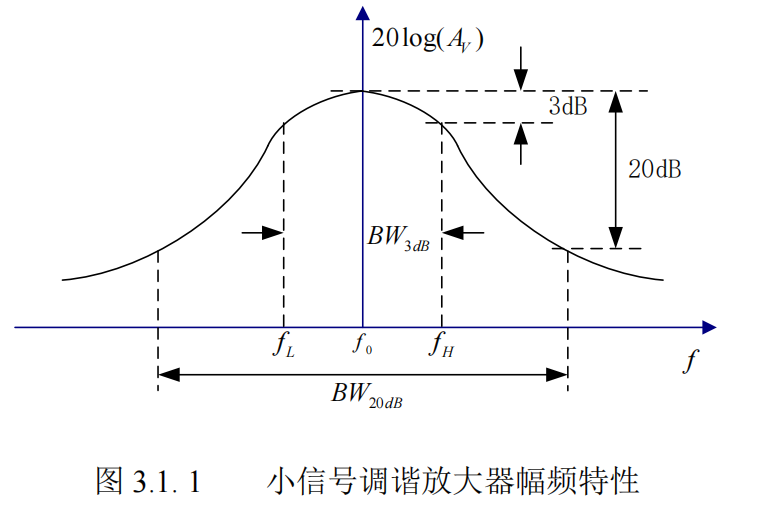
\includegraphics[scale=0.4]{pic/fig1.png}
            \caption{1dB 增益压缩点}
        \end{figure}

        \subsection{AGC主要性能指标}

        (1) 动态范围: 在给定输出信号幅值变化的范围内,容许输入信号振幅的变化越大,则表明 AGC 电路的动态范围越宽,性能越好。AGC 电路的动态增益范围就是输入动态范围与输出动态范围之比,也称为放大器的增益控制倍数,用 MAGC 表示
        
        $$
        \begin{aligned}
            MAGC &=& Di − Do = (Pi max − Pi min) − (Po max − Po min)
            &=& (Po min − Pi min) − (Po max − Pi max) = Gmax − Gmin    
        \end{aligned}
        $$

        可见,要扩大 AGC 电路的控制范围,就要增大 AGC 电路的增益控制倍数 M AGC ,也就是要求 AGC电路有较大的增益变化范围。增加 AGC 电路控制的级数可以扩大 AGC 电路的控制范围。

        (2) 响应时间: 需要根据信号的性质和需要,设计适当的响应时间。可采用调节环路带宽,主要是调节低通滤波器的带宽的方式调整响应时间,一般上限频率设计为 10 \~ 20Hz。



    \section{实验电路分析}

        \begin{figure}[H]
            \centering
            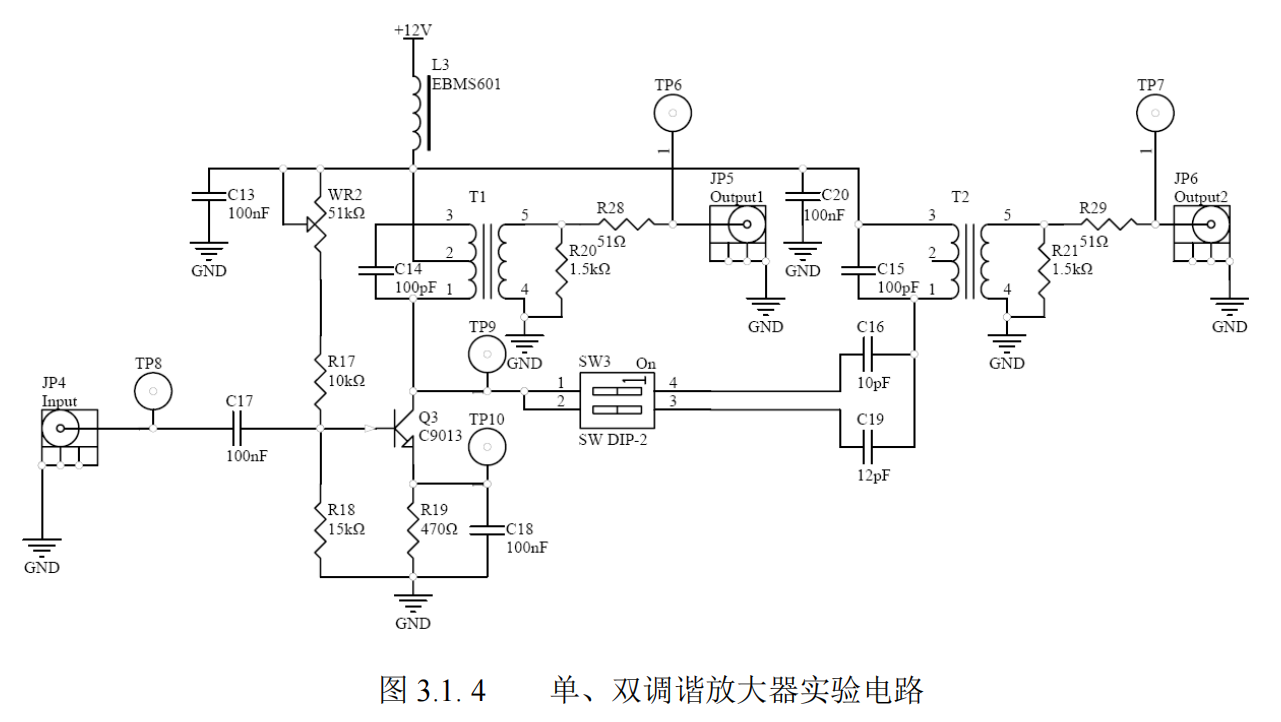
\includegraphics[width = 0.8\textwidth]{pic/fig2.png}
            \caption{两级级联 AD603 放大器}
        \end{figure}

        电路中两个 AD603 放大器级联,由电容 C9 耦合。采用顺序增益控制方式,两放大器 GNEG 管脚间的电压差为 1V 左右,由电阻 R13、R14、R15 分压得到。两放大器的增益分别由 R7、R8 确定,本实验电路中取
        值为 2.5kΩ,则单级最大增益约为 42dB,因此电路的最大增益可达 84dB。通过选取合适的 R7、R8,增益控制范围可在 20dB 内变动。电路中 Q2 和 R6 构成一个检波器,用于检测放大器输出信号幅度的变化;Q1 和外围电阻构成一个简单的恒流源电路,其集电极电流保持基本不变;流入电容 C4 的电流是 Q1 与 Q2 集电极电流的差值,Q2 集电极的电流随着输出信号幅度的增加而增加。自动增益控制电压 VAGC 是这个差值的时间积分,因此它随输出信号幅度的变化而变化,从而达到自动调整放大器增益的目的。电路稳定时,Q2 检波电流的平均值要与 Q1 的电流平衡。如果放大器输出幅度太小不能满足这个条件,VAGC 会增加,使得放大器增益增加,输出幅度变大,直到 Q2 与 Q1 的平均电流达到平衡。开关 SW4 及外围的电阻网络构成一可变衰减器。
        SW4 控制对输入信号的衰减量,设为“1000”(即接通第一路开关),衰减 0dB;设为“0100”,衰减 20dB;设为“0010”,衰减 40dB;设为“0001”,衰减 60dB;设为“0000”,衰减 80dB。开关 SW2 用以控制 AGC 环
        路。当开关 SW2 处于断开(Open)状态时,整个放大电路处于开环状态,增益由可变电阻 WR1 控制。当开关 SW2 处于闭合(Close)状态时,整个放大电路处于闭环状态,可以实现自动增益控制功能。


    \section{实验设备}
        \begin{enumerate}
            \item 实验办No01 \, 1块
            \item 信号源1台
            \item 双踪示波器1台
            \item 频谱分析仪(含TG)1台
            \item 外用表1台
        \end{enumerate}
        
    \section{实验数据与结果分析}
        \subsection{开环放大器的测量}
            \subsubsection{最大开环增益的测量}
            
            高频信号源的输出连接到实验板的 JP2;设定高频信号源产生幅值为-40dBm,频率为 10.7MHz 的正弦信号;设定频谱分析仪的中心频率为 10.7MHz,扫描宽度为 100KHz,调节可变电阻 WR1,使输出信号最大且不失真, 其测量结果如下图:

            \begin{figure}[H]
                \centering
                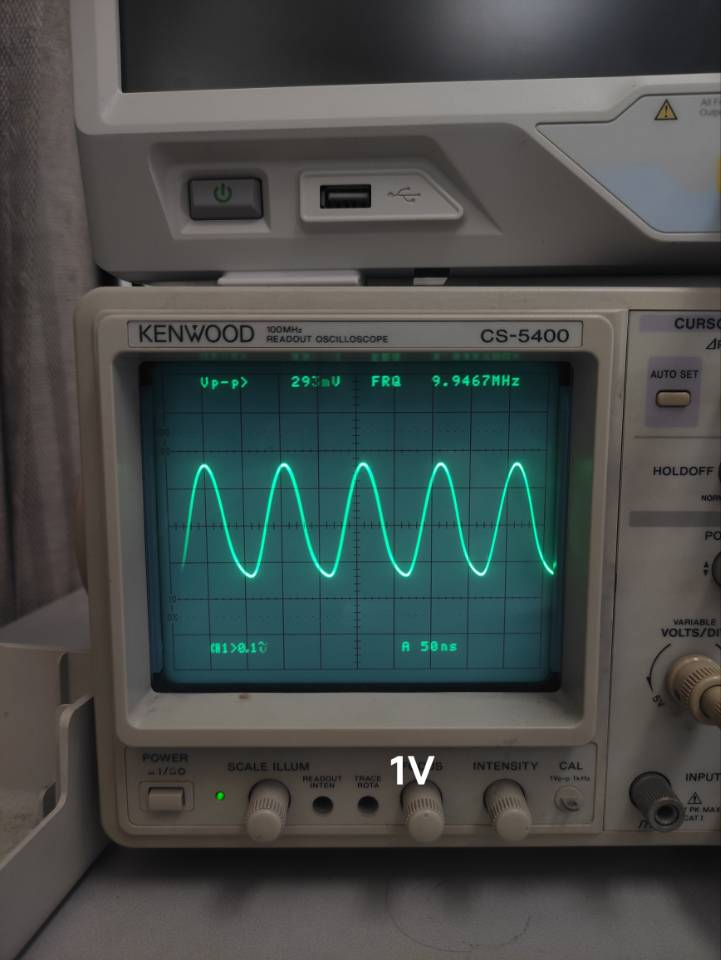
\includegraphics[width = 0.6\textwidth]{4}
                \caption{输出信号}
            \end{figure}

            可以从图中读出,信号峰值为-5.91dBm,又因为前面设置了输入信号衰减 40dB,因此最大增益 G=(-5.91)-(-40)+40=74.09dB。


            
            \subsubsection{噪声系数 NF 的测量}

            将电路板输入端与高频信号源断开,接 50Ω 电阻;设定可变衰减器衰减为 0dB(将 SW4 设为“1000”);设定频谱分析仪扫描带宽为 100KHz,分辨率带宽为 100Hz,参考电平为-40dBm。用频谱分析仪测量放大器在10.7MHz 频率点上的噪声功率值。测量结果如下图

            \begin{figure}[H]
                \centering
                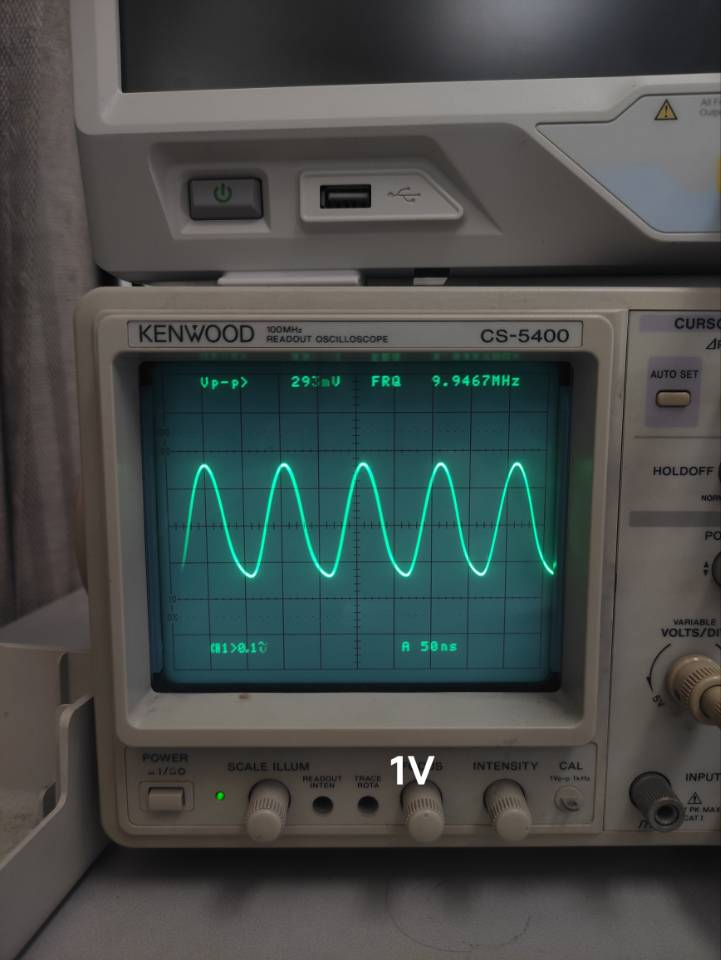
\includegraphics[width = 0.6\textwidth]{4}
                \caption{噪声功率}
            \end{figure}

            
            可以从图中读出,10.7MHz 频率点上的噪声功率值为-73.29dBm。根据公式 NF(dB) = Nout(dBm/RBW)−
            10 log(RBW) + 174dBm/Hz − Gain(dB) 可以算出 NF(dB)=-73.29-10log(100)+174-74.09=6.62dB 噪声系数
            应当越小越好,本电路的噪声系数较大。
            
            
            \subsubsection{1dB 增益压缩点的测量}

            首先需要设定放大电路的增益,具体步骤为:设定可变衰减器衰减为 40dB(将 SW4 设为“0010”);在 JP2端由高频信号源输入大小为 0dBm,频率为 10.7MHz 的正弦信号;调节可变电阻 WR1,使 JP3 端输出信号大小为 0dBm,则此时放大器的增益为 40dB。进行 1dB 压缩点测量时,调整高频信号源的输出功率在 0dBm 至20dBm 之间变化(实际输入在-40dBm 至-20dBm 之间变化),以 1dBm 为步进。

            \begin{figure}[H]
                \centering
                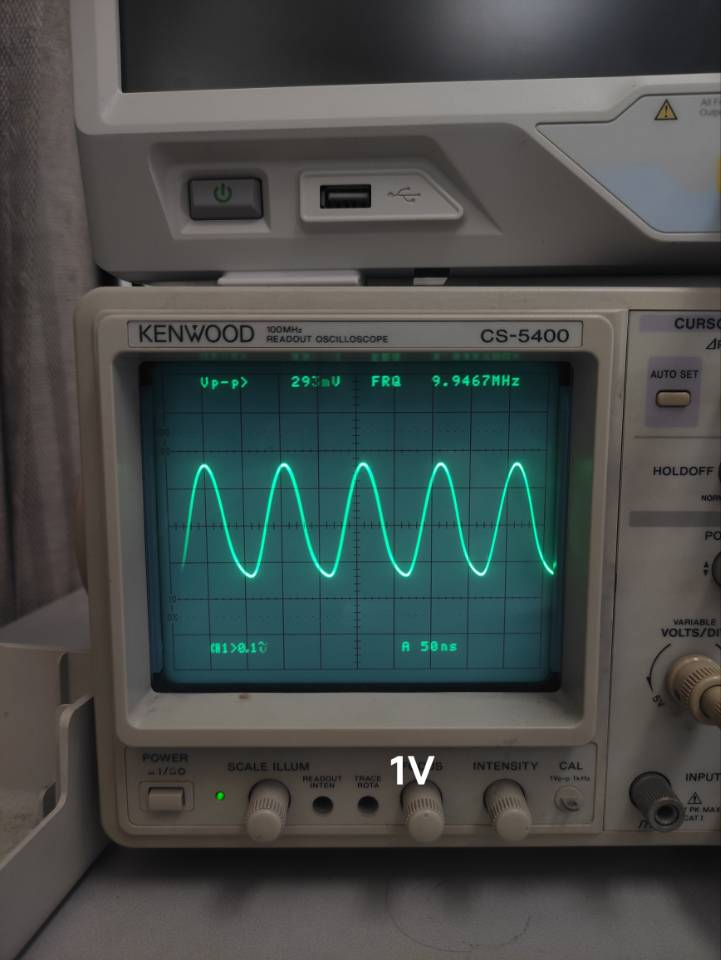
\includegraphics[width = 0.6\textwidth]{4}
                \caption{高频信号从 0dBm 至 20dBm 依次测量,示意图为 1dBm 时}
            \end{figure}

            \begin{figure}[H]
                \centering
                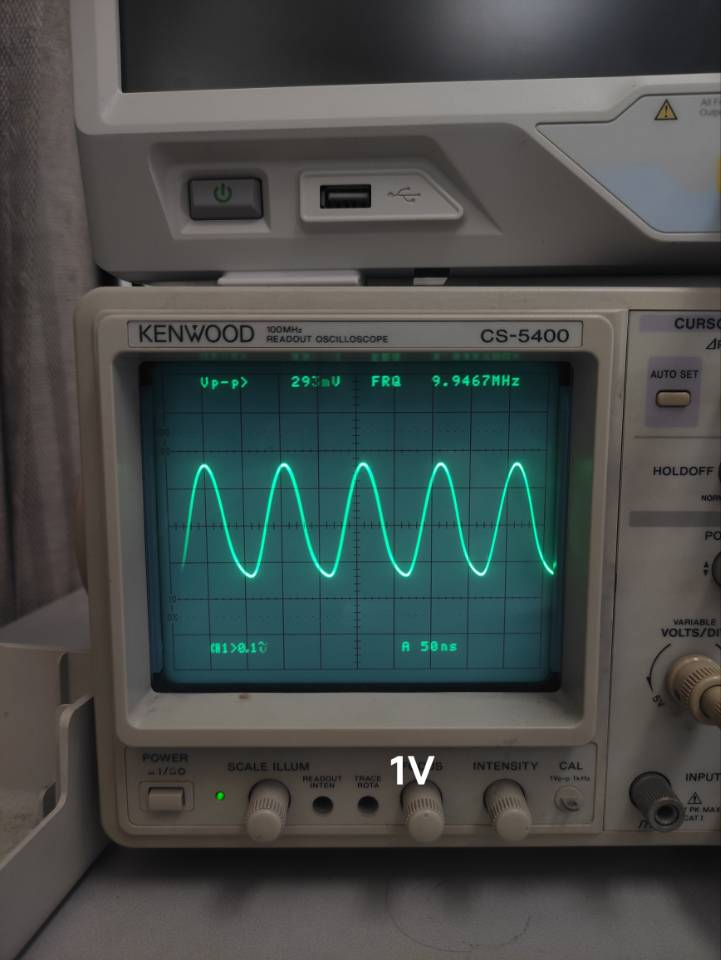
\includegraphics[width = 0.6\textwidth]{4}
                \caption{高频信号 1dBm 时测量结果示意}
            \end{figure}

            记录对应的输入、输出信号功率值,填入下表:

            \begin{table}[H]
                \begin{tabular}{|c|c|c|c|c|c|c|c|c|c|c|}
                \hline
                输入功率(dBm) & -40  & -39   & -38   & -37  & -36   & -35   & -34  & -33   & -32   & -31   \\ \hline
                输出功率(dBm) & 0    & 0.98  & 1.86  & 2.7  & 3.47  & 4.32  & 5.2  & 6.03  & 6.89  & 7.62  \\ \hline
                增益(dB)    & 40   & 39.98 & 39.86 & 39.7 & 39.47 & 39.32 & 39.2 & 39.03 & 38.89 & 38.62 \\ \hline
                输入功率(dBm) & -30  & -29   & -28   & -27  & -26   & -25   & -24  & -23   & -22   & -21   \\ \hline
                输出功率(dBm) & 8.1  & 8.42  & 8.57  & 8.7  & 8.76  & 8.81  & 8.8  & 8.8   & 8.73  & 8.73  \\ \hline
                增益(dB)    & 38.1 & 37.42 & 36.57 & 35.7 & 34.76 & 33.81 & 32.8 & 31.8  & 30.73 & 29.73 \\ \hline
                \end{tabular}
                \end{table}

            从上表中可以看出,刚开始随着输入功率的增大,增益基本上为恒定值在 40dB 左右,然后到输入功率增
            大到-32dBm 时输出功率为 6.89dBm,增益仅为 38.89dBm,该点为 1dB 压缩点。小于该点的输入功率的小信
            号会工作在线性区域。

        \subsection{AGC放大器特性测量}

            将开关 SW2 置于闭合状态,则放大器处于自动增益控制状态。当输入信号小于一定幅度时,AGC 放大器增益达到最大。随着输入信号的加大,放大器的增益逐渐减小,输出信号幅度保持基本不变。测量时,将输入信号衰减器设定为衰减 20dB;在 JP2 端由高频信号源输入大小为-50dBm,频率为 10.7MHz 的正弦信号,以10dBm 为步进增加输入信号的功率,直到 30dB。

            \begin{figure}[H]
                \centering
                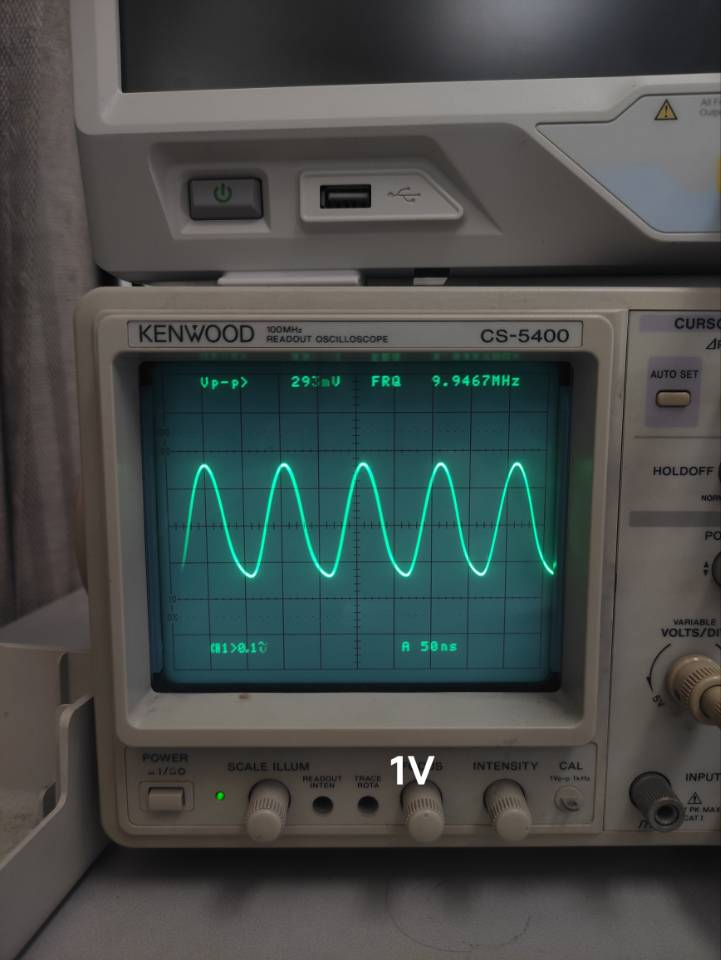
\includegraphics[width = 0.6\textwidth]{4}
                \caption{因为最后无法达到 30dBM , 最后到 24dBm 左右为止}
            \end{figure}

            用频谱分析仪和示波器观察输出信号的大小,当输出信号功率不随输入信号功率的增加而增加时,放大器自动增益控制开始发挥作用。记录输入信号功率与输出信号功率填入下表:

            \begin{table}[H]
                \begin{tabular}{|c|c|c|c|c|c|c|c|c|c|}
                \hline
                输入功率(dBm) & -70   & -60   & -50   & -40   & -30   & -20   & -10   & 0    & 3.98  \\ \hline
                输出功率(dBm) & 2.07  & 3.17  & 3.17  & 3.35  & 3.63  & 3.66  & 3.61  & 3.63 & 3.66  \\ \hline
                增益(dB)    & 72.07 & 63.17 & 53.17 & 43.35 & 33.63 & 23.66 & 13.61 & 3.63 & -0.32 \\ \hline
                \end{tabular}
            \end{table}

            从上表中可以看出,在输入信号为-70dBm 到-60dBm 增加时,输出信号有 1 dBm 左右的增加,当输入信号大于-60dBm 时随着输入信号的逐渐增大,输出信号功率趋近于稳定不变, 实现了自动增益控制。其最大增益 Gmax = 72.07dB,Gmin = −0.32dB, 动态范围 MAGC =-0.32dB 72.07dB。

    \section{思考题}
	    \subsection{低噪声放大器的主要性能指标有哪些?}
       
        \subsection{结合实验电路,简述自动增益控制放大器的电路工作原理。
        }
        
        \subsection{实验电路中,为何要在放大器输入端设置可变衰减器?}
	
\end{document}